\chapter{Design}

\section{A Buffalo Example}

An example of how to use Buffalo is presented in Listing~\ref{aspectexample}. Further detail on the design will be discussed in later sections. The example shows how a simple aspect is created. It inherits MethodBoundaryAspect, which is a predefined aspect by Buffalo, and overrides its OnBefore and OnAfter functions.

\begin{minipage}{\textwidth}
\begin{lstlisting}[caption={Sample TraceAspect}, label=aspectexample]
using Buffalo;
using System;
public class TraceAspect : MethodBoundaryAspect
{
    public override void OnBefore(MethodArgs args)
    {
        Display("ENTERING", args);
    }
    public override void OnAfter(MethodArgs args)
    {
        Display("EXITING", args);
    }
    void Display(string title, MethodArgs args)
    {
        Console.WriteLine("{0} {1}", title, args.FullName);
        foreach (var p in args.Parameters){
            Console.WriteLine("\t{0} ({1}) = {2}", 
			p.Name, p.Type, p.Value);
        }
    }
}
\end{lstlisting}
\end{minipage}

To use the aspect, simply apply it to a method, class or assembly. This ensures that whenever a public function of a class attributed with TraceAspect is invoked, OnBefore and OnAfter of the aspect will be invoked respectively. Once the code is compiled to produce an assembly, BuffaloAOP.exe can be invoked by passing it the path to the assembly. Buffalo will take over and weave in the aspect. This and more examples and details are also provided in Appendix A.

\begin{minipage}{\textwidth}
\begin{lstlisting}[caption={Apply Aspect on Class Level}, label=helloaspect]
[TraceAspect]
public class Hello
{
    //...
}
\end{lstlisting}
\end{minipage}

\section{Usage Comparison With AspectJ and PostSharp}

What functionality does Buffalo support? What type of weaving does it do? For inspiration, existing works, such as AspectJ~\cite{aspectj_faq} and PostSharp~\cite{postsharp}, were studied. Specifically, Buffalo will intercept the various points of an executing method. Those points are namely the following: before a method executes; after a method executes; whether the method executed successfully without error or the method throws an exception at any point during the execution. These various points of interception are grouped into the MethodBoundaryAspect.

Buffalo is influenced by AspectJ and PostSharp. PostSharp makes use of System.Attribute as well, and the creation and usage of aspect is similar to Buffalo. A simple example to replace a function call foo() is presented below to illustrate some of the similarities and differences.

Listing~\ref{buffaloaround} shows that Buffalo creates an aspect inheriting from MethodAroundAspect, which is one of the predefined aspects in Buffalo. It overrides the Invoke(), so anytime the annotated function foo() is invoked, the aspect will be called to return 3 instead of 100.

\begin{minipage}{\textwidth}
\begin{lstlisting}[caption={Buffalo MethodAroundAspect}, label=buffaloaround]
public class MyAspect : MethodAroundAspect
{
    public override object Invoke(Buffalo.MethodArgs args)
    {
        return 3;
    }
}

public class Program
{
    [MyAspect]
    public int foo(){
        return 100;
    }
}
\end{lstlisting}
\end{minipage}

AspectJ is a compiler that produces compatible Java bytecode. It has its own syntax that is somewhat different from Java. Listing~\ref{aspectjaround} defines an aspect that will replace all the calls to foo() and returns the integer 3 instead.

\begin{minipage}{\textwidth}
\begin{lstlisting}[caption={AspectJ Around}, label=aspectjaround]
aspect A {
    int around(): call(int foo()) {
        return 3;
    }
}
\end{lstlisting}
\end{minipage}


Listing~\ref{postsharpintercept} shows an example of PostSharp, which is very similar to how Buffalo is used. The big difference is that the return value is carried in the argument object instead of returning it directly.

\begin{minipage}{\textwidth}
\begin{lstlisting}[caption={PostSharp MethodInterceptionAspect}, label=postsharpintercept]
[Serializable]
public class MyAspect : MethodInterceptionAspect
{
    public override void OnInvoke(MethodInterceptionArgs args)
    {
        args.ReturnValue = 3;
    }
}

public class Program
{
    [MyAspect]
    public int foo()
    {
        return 100;
    }
}
\end{lstlisting}
\end{minipage}

Functionally, AspectJ and PostSharp are closely matched, but with some strong differences in the approach of implementation.

\begin{enumerate}
	\item The most noticeable is the approach to pointcuts. AspectJ has a rather elaborate syntax language for defining pointcuts. Whereas PostSharp and Buffalo’s approach is a basic declarative system, making use of the attribute system in .NET.

	\item There is conditional pointcuts in AspectJ. This is not supported in either PostSharp or Buffalo.

	\item On the other hand, PostSharp and Buffalo support events and properties automatically, since at compile time those were transformed into methods by the compiler. AspectJ has the get() and set(), but they rely on pattern matching to find the properties.

	\item Both AspectJ and PostSharp provide a set of tools that integrate into Eclipse and Visual Studio respectively, to make development a lot more visual and easy.

	\item AspectJ, PostSharp and Buffalo all support aspect composition, where multiple aspects can be applied to the same join point. Although in Buffalo the ordering of the execution is not enforced.

\end{enumerate}


%\pagebreak
\section{Aspect Interface}

Figure~\ref{uml01} shows the relationship of various aspect types in Buffalo. This is used by Buffalo to identify aspects during reflection.

\begin{figure}[H]
  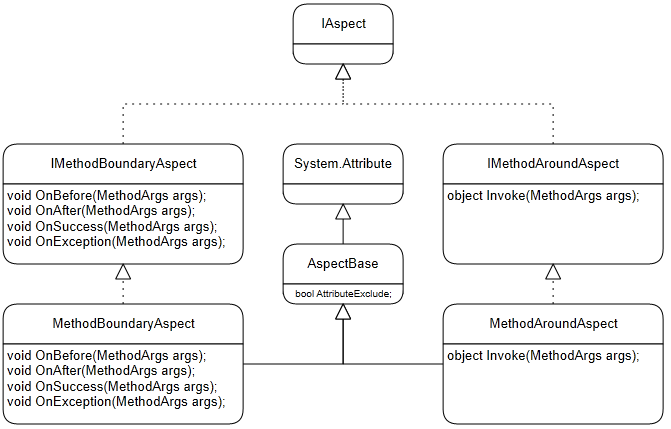
\includegraphics[scale=1.0]{Uml02.PNG}
  \centering
  \caption{Aspect Inheritance\label{uml01}}
\end{figure}

All aspects ultimately implement the IAspect interface; therefore, it can be reasoned that for all the public types in an assembly that if a type implements IAspect, then it must be an aspect itself.

Buffalo supports more than one aspect applied at any given level. This will allow developers more flexibility while developing multiple aspects and applying them as needed.

Furthermore, by default, an aspect will be automatically excluded from applying to itself. This is implemented to prevent unintended recursion in some cases. Although argument can be made that an aspect should be able to be applied to a different aspect; that is not currently implemented in Buffalo.



\section{MethodArgs}

As mentioned above, when all is said and done, an aspect ultimately gets injected into each \textit{individual} method. When developing an aspect, meta-information about the target method can be accessed. This information is encapsulated via the MethodArgs object passed in as parameter to the aspect. Method name, its full method signature, return type and parameter list (including parameter name, type and value) are captured for each target method.

The parameter list capturing is especially of interest; it enables the developer to peek inside the method that is executing at various point and inspect its parameter values. This will be useful in cases such as exception handling, where it will be useful to see what the actual values were at the time of the exception. When using MethodAroundAspect, the parameter values can even be modified and passed back to the original method.


\section{A Buffalo Aspect}

When performing Post Compilation Weaving, Buffalo must have the ability to discover what aspect is applied to what methods in an assembly. In order to achieve that, the target assembly has to carry some identifying meta-data.

A given .NET assembly already carries a great deal of such meta-data for various purposes. .NET has the System.Attribute type that exists primarily for the purpose of inserting meta-data into the assembly during compilation. When the source code is compiled, it is converted into CIL~\cite{msil_text} and put inside a portable executable (PE) file, with the meta-data generated by the compiler. 

Buffalo takes advantage of this characteristic in two phases.
\begin{enumerate}
	\item An aspect defined in Buffalo will be in the form of an attribute by inheriting from System.Attribute. It can, therefore contain any valid .NET code. Specifically, however, an aspect needs to override various predefined methods in order to do something useful.
	\item After compilation, the assembly will now contain the meta-data about all the aspects. Buffalo can inspect the assembly for such information and perform CIL code injection accordingly.
\end{enumerate}

In other words, a Buffalo aspect is a .NET attribute in disguise.

\section{MethodBoundaryAspect}
MethodBoundaryAspect can be cleanly mapped to the try-catch-finally statements of the .NET languages. As far as the runtime is concerned~\cite{ecma334, ecma335}, try-catch can be used liberally without serious performance degradation. For example, a simple method is shown in Figure~\ref{samplefunction}:

\begin{minipage}{\textwidth}
\begin{lstlisting}[caption={Sample Function}, label=samplefunction]
public void SomeFunction () {
    //Perform some action...
}
\end{lstlisting}
\end{minipage}

When performing CIL modification, the above will be transformed by Buffalo into something shown in Figure~\ref{sampletcf}. This clearly captures the spirit of the MethodBoundaryAspect. Regardless of whether the source already contains its own try-catch, or try-catch-finally blocks, Buffalo will wrap the body of the method inside of a new try-catch-finally block.

\begin{minipage}{\textwidth}
\begin{lstlisting}[caption={Sample Try-catch-finally}, label=sampletcf]
public void SomeFunction () {
    try {
        OnBefore();
        //Perform some action
        OnSuccess();
    }
    catch (Exception e) {
        OnException(e);
    }
    finally {
        OnAfter();
    }
}
\end{lstlisting}
\end{minipage}

The transformed method in Figure~\ref{sampletcf} still does what the original method intends to do; only now at various points, execution is being intercepted to provide more functionality. 

\section{MethodAroundAspect}
Another type of aspect that Buffalo supports is the MethodAroundAspect. Rather than intercepting various execution points of a method, the method can be completely replaced by another method defined in an aspect while preserving the option to call back into the original method if necessary.

At first glance MethodAroundAspect sounds straightforward to implement, but it turns out to be much more involved than the MethodBoundaryAspect.

Since the option to call back into the original method is needed, it is critical that the original method is not modified under any circumstance. If the method body instructions are simply overridden with that of the replacement, the call back to the original method will be meaningless since the method is now changed. The original method must stay intact during the CIL modification.

To get around this obstacle, whenever Buffalo encounters the MethodAroundAspect applied to a method, it dynamically generates a replacement method in CIL with the same method signature as the original.

The body of this replacement method is also completely different than the original. It instantiates the aspect and makes a call to the Invoke() method, which is the actual code that will be run as a replacement. 

Inside the Invoke method, the developer can issue a call back to the original method via a call to the Proceed() method. Then throughout the program, for any calls made to the original method, Buffalo will change them to call the replacement method instead. This process is illustrated in Figure~\ref{around_overview}.

\begin{figure}[H]
  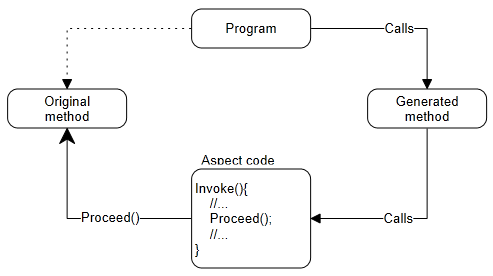
\includegraphics[scale=1.0]{AroundOverview3.PNG}
  \centering
  \caption{Illustration of MethodAroundAspect\label{around_overview}}
\end{figure}

The dotted line from Program to the original method indicates that once the MethodAroundAspect is applied to it, from the perspective of CIL the program cannot directly access that method any more. Access to the original method now must come from inside the aspect. Also note that the original method is not changed at any given time.


\section{How to Apply an Aspect}

Since an aspect is really a .NET attribute, it can be used just like any other attribute. However, code annotated with an aspect is special in that it can be understood only by Buffalo.

A Buffalo aspect can be applied on three levels, with the following characteristics:

\begin{enumerate}
  \item Method - apply the aspect to an individual method.
  \item Class - if aspect is applied to a class, all public methods, including the public properties, are automatically applied.
  \item Assembly - if aspect is applied to an assembly, \#2 will apply for all of the public classes within the assembly.
\end{enumerate}

MethodAroundAspect, however can only be applied on a method level, as will be shown later.

All aspects have a property named AttributeExclude; if this property is set to true, then the annotated target will not be included in the weaving. This exclusion can happen on any level. For example, if a method contains this annotation [SampleAspect(AttributeExclude=true)], the method will be skipped for the SampleAspect during the weaving process.

No matter how the aspect is applied, ultimately it will result in a list of the methods that are annotated. This simply means that if the aspect is applied to a single method, that method is the only one that will get CIL modified. If the aspect is applied on the whole assembly, then all public methods will be CIL modified.

To get the list of the eligible methods for CIL modification, Buffalo attempts various checking according to Figure~\ref{logical_inclusion} to see if it should include a given method.

\begin{figure}[H]
  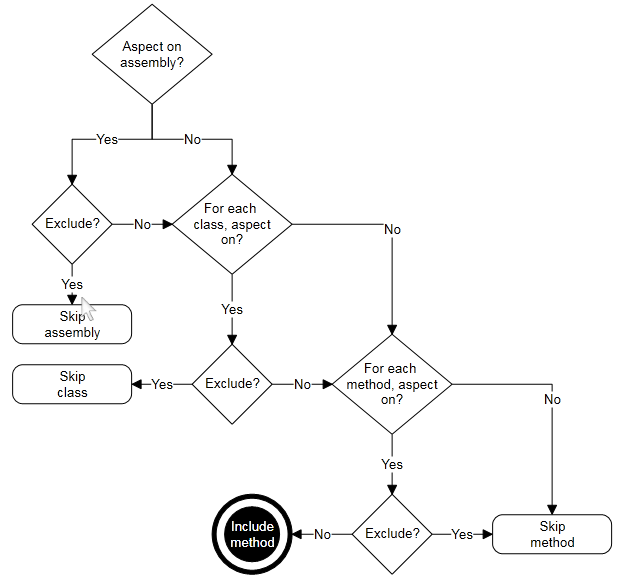
\includegraphics[scale=1.0]{AspectLogicalInclusion2.PNG}
  \centering
  \caption{Diagram for Finding Eligible Methods\label{logical_inclusion}}
\end{figure}

If no aspect is applied on the assembly, it does not necessarily mean no aspect is applied anywhere; the aspect might still be applied on any given class or method.

Buffalo first checks if an aspect is applied to the target, and then checks if it is set to be excluded. At the end it will end up with a list of methods that should be CIL modified.


\section{Visual Studio Solution Structure}

Originally Buffalo was implemented as one executable; that includes the various aspects and the program that initiates the weaving. It was later separated into two assemblies. One is a class library that contains the actual implementation. Another is a command line executable that calls into the class library to perform the weaving. This separation is necessary so that the developer can perform weaving from the command line or hook into MS-Build if necessary. 

To actually write the aspect, one only needs to reference the class library as underlined in Figure~\ref{solutionexplorer}.

\begin{figure}[H]
  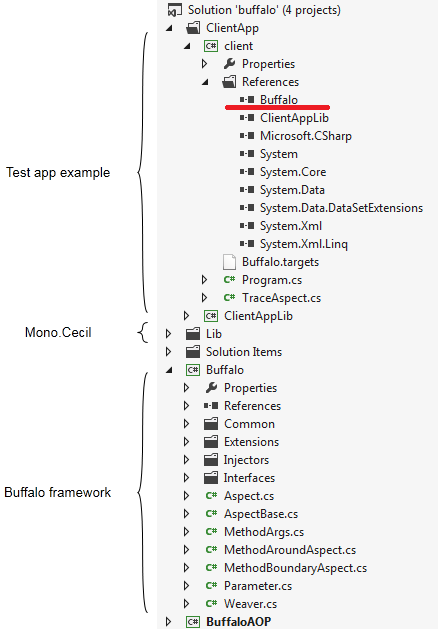
\includegraphics[scale=1.0]{SolutionExplorer3.PNG}
  \centering
  \caption{Solution Structure\label{solutionexplorer}}
\end{figure}

The client project shown above is a simple program included in the solution for testing.
